\chapter{Additional results}
\label{ch:additional}

% Appendix containing reliability diagrams per model, per-fold
% curves from K-fold CV, full conformal results, etc.

\section{Reliability diagrams (binary models)}
% \begin{figure}[h]
%   \centering
%   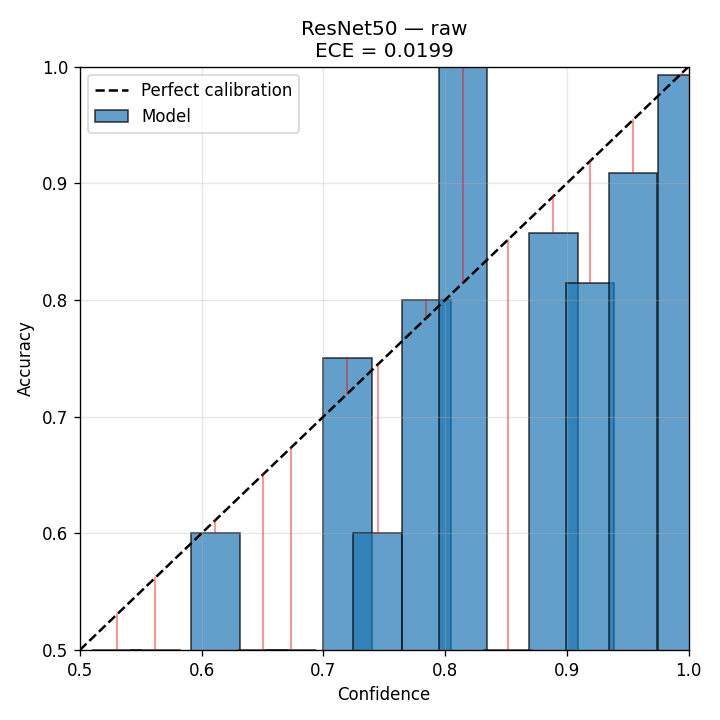
\includegraphics[width=0.45\linewidth]{../results/reliability_ResNet50_raw.png}
%   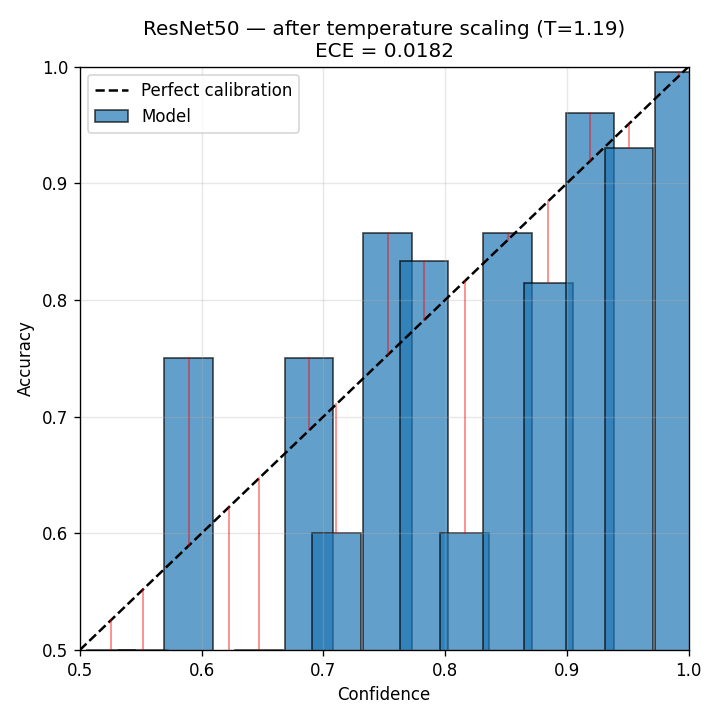
\includegraphics[width=0.45\linewidth]{../results/reliability_ResNet50_temp_scaled.png}
%   \caption{ResNet50 reliability before (left) and after (right) temperature scaling.}
% \end{figure}
% Repeat for Xception, DenseNet121, VGG16, CNN, CNN(Tanh+ReLU), Ensemble.

\section{Reliability diagrams (5-class)}
% Include cnn\_5class and resnet50\_5class reliability diagrams.

\section{Confusion matrices (5-class)}
% 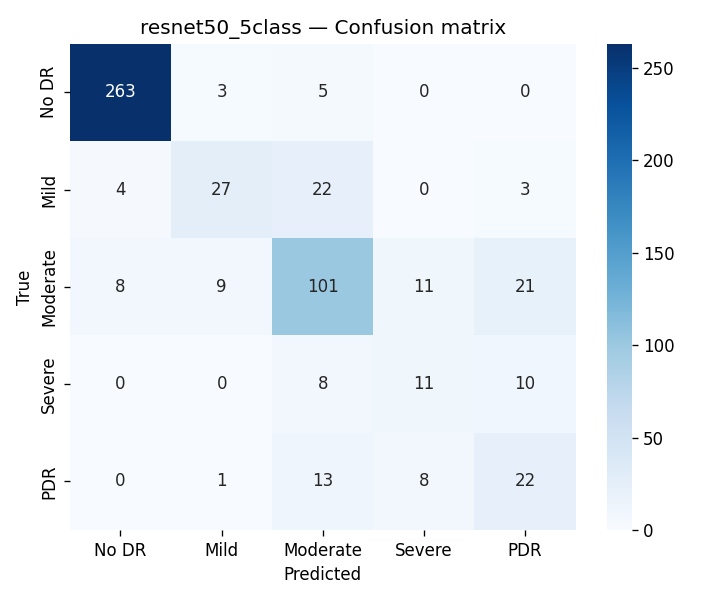
\includegraphics[width=0.6\linewidth]{../results/multiclass/resnet50_5class_confusion_matrix.png}

\section{Per-fold history curves (K-fold CV)}
% Optionally include per-fold val loss/accuracy curves saved by run\_kfold\_cv.py.

\section{Per-class conditional coverage tables}
% Full conformal CSVs (master/results/multiclass/) reproduced verbatim.

\section{Phase 1 reliability diagrams (full)}
% Optional: include all 14 reliability PNGs (raw + temp-scaled per model).
